
%\newtheorem{definition}[subsection]{Definition}
%\newtheorem{example}[subsection]{Example}
\newtheorem{cor}[subsection]{Corollary}
\newtheorem{pro}[subsection]{Proposition}
\newtheorem{theo}[subsection]{Theorem}
\newtheorem{lem}[subsection]{Lemma}
%\newtheorem{rem}[subsection]{Remark}

\definecolor{main}{HTML}{5989cf}    % setting main color to be used
\definecolor{sub}{HTML}{cde4ff}     % setting sub color to be used

\tcbset{
    sharp corners,
    colback = white,
    before skip = 0.2cm,    % add extra space before the box
    after skip = 0.5cm      % add extra space after the box
}                           % setting global options for tcolorbox

% You can copy any following box you like to your code.
\newtcolorbox{boxA}{
    fontupper = \bf,
    boxrule = 1.5pt,
    colframe = black % frame color
}

\newtcolorbox{boxB}{
    fontupper = \bf\color{main}, % font color
    boxrule = 1.5pt,
    colframe = main,
    rounded corners,
    arc = 5pt   % corners roundness
}
\newtcolorbox{boxC}{
    colback = sub, % background color
    boxrule = 0pt  % no borders
}

\newtcolorbox{boxD}{
    colback = sub, 
    colframe = main, 
    boxrule = 0pt, 
    toprule = 3pt, % top rule weight
    bottomrule = 3pt % bottom rule weight
}

\hypersetup{
    colorlinks=true,
    linkcolor=blue,
    filecolor=magenta,      
    urlcolor=cyan,
    pdftitle={Overleaf Example},
    pdfpagemode=FullScreen,
    }

\urlstyle{same}


\coursetitle{\mtthreeiii}{MT303}
\developers{Wyclife Rao}
\reviewers{Dr Irene Sitawa}
\modulenumber{10}
\modulename{Numerical Methods for Ordinary Differential Equations Using Python}

% courses
\thispagestyle{empty}
\begin{tikzpicture}[overlay,remember picture,font=\sffamily\bfseries]
 \draw[ultra thick,c4,name path=big arc] ([xshift=-2mm]current page.north) arc(150:285:11) coordinate[pos=0.225] (x0);
 \begin{scope}
  \clip ([xshift=-2mm]current page.north) arc(150:285:11) --(current page.north east);
  \fill[c4!50,opacity=0.25] ([xshift=4.55cm]x0) circle (4.55);
  \fill[c4!50,opacity=0.25] ([xshift=3.4cm]x0) circle (3.4);
  \fill[c4!50,opacity=0.25] ([xshift=2.25cm]x0) circle (2.25);
  \draw[ultra thick,c4!50] (x0) arc(-90:30:6.5);
  \draw[ultra thick,c4] (x0) arc(90:-30:8.75);
  \draw[ultra thick,c4!50,name path=arc1] (x0) arc(90:-90:4.675);
  \draw[ultra thick,c4!50] (x0) arc(90:-90:2.875);
  \path[name intersections={of=big arc and arc1,by=x1}];
  \draw[ultra thick,c4,name path=arc2] (x1) arc(135:-20:4.75);
  \draw[ultra thick,c4!50] (x1) arc(135:-20:8.75);
  \path[name intersections={of=big arc and arc2,by={aux,x2}}];
  \draw[ultra thick,c4!50] (x2) arc(180:50:2.25);
 \end{scope} 
 \path[decoration={text along path,text color=c4,
                 raise = -2.8ex,
                 text  along path,
                 text = {},%|\sffamily\bfseries|02/18/2019
                 text align = center,
             },
             decorate
         ] ([xshift=-2mm]current page.north) arc(150:245:11);
 %
 \newcommand\add{4cm}
 \begin{scope}%[shift={(5,0)}]
  \path[clip,postaction={fill=c3}]
  ([xshift=2cm+\add,yshift=-8cm]current page.center) rectangle ++ (4.6,7.7);
  \draw[c5,ultra thick,fill=c2] ([xshift=0.5cm+\add,yshift=-8cm]current page.center)
   ([xshift=0.5cm+\add,yshift=-8cm]current page.center)  arc(180:60:2)
    |- ++ (-3,6) --cycle;
  \draw[ultra thick,c5] ([xshift=-1.5cm+\add,yshift=-8cm]current page.center) 
  arc(180:0:2);
  \draw[ultra thick,c5] ([xshift=0.5cm+\add,yshift=-8cm]current page.center) 
  arc(180:0:2);
  \draw[ultra thick,c5] ([xshift=2.5cm+\add,yshift=-8cm]current page.center) 
  arc(180:0:2);
  \draw[ultra thick,c5] ([xshift=4.5cm+\add,yshift=-8cm]current page.center) 
  arc(180:0:2);
  \fill[white] ([xshift=2.5cm+\add,yshift=-8cm]current page.center) +(60:2) circle(1.5mm)
  node[above
  right=0mm,text=c5!80!black]{$\rho:=\dfrac{1+\sqrt{-3}}{2}$};
 \end{scope}
 %
 \fill[c1] ([xshift=2cm+\add,yshift=-8cm]current page.center) rectangle ++ (-30.7,7.7);
 \node[text=white,anchor=west,scale=2.3,inner sep=0pt] at
 ([xshift=-10cm,yshift=-1.8cm]current page.center) {\color{ulabgold} LEARNING};
 \node[text=white,anchor=west,scale=5,inner sep=0pt] at
 ([xshift=-10cm,yshift=-3.25cm]current page.center) {MODULE \dpmdnumber};
 \node[text=white,anchor=west,scale=2.5,inner sep=0pt,text width=.4\textwidth] at
 ([xshift=-10cm,yshift=-6cm]current page.center) {\dpmdname};
 \node[text=white,anchor=east,scale=2,inner sep=0pt] at
 ([xshift=5.7cm,yshift=-7.5cm]current page.center) {\color{ulabgold}The Open University of Kenya};
 %
% \draw[gray,line width=5mm] 
% ([xshift=2mm,yshift=-1mm]current page.south west) rectangle ([xshift=-2mm,yshift=1mm]current
% page.north east);
\end{tikzpicture}

%\newpage
\pagenumbering{roman}
\thispagestyle{empty}%firstpage


\begin{center}
\vspace*{2cm}
{\Huge\bf BACHELOR OF TECHNOLOGY EDUCATION}\\[3cm]  


%{\fontsize{80}{40}\selectfont \dpcoursecode}\\[2cm]
%
%{\fontsize{30}{40} \selectfont \dpcoursename}\\[2cm]

%\rule{\textwidth}{1pt}
%\vspace{2cm}

%{\fontsize{40}{40}\selectfont \bf Module~\dpmdnumber}\\[2cm]
%
%{\fontsize{30}{40}\selectfont \bf \dpmdname}\\

\vfill
\begin{flushright}
\begin{minipage}{.6\textwidth}
\begin{tcolorbox}%[text ]
\begin{tabular}{ll}%\hline
\subtitle{Developed by:}&\displaydevelopers\\
&\\
\subtitle{Reviewed by:}&\makecell[l]{\displayreviewers}\\
\end{tabular}
\end{tcolorbox}
\end{minipage}\hspace*{-3.5cm}
\end{flushright}
\vspace*{-2.5cm}
\end{center}

\newpage
\thispagestyle{empty}
\null
\vfill
{\renewcommand\arraystretch{1.5}
\begin{tabular}{|l|l|}\hline
\subtitle{Programme Title} & Bachelor of Technology Education \\\hline
\subtitle{Course Title} & \fullcoursename\\\hline
\subtitle{Learning Module number} & Module \dpmdnumber\\\hline
\subtitle{Learning module title} & \dpmdname \\\hline
\subtitle{Module Developer} & \displaydevelopers\\\hline
\subtitle{Reviewed by} & \displayreviewers\\\hline
%\subtitle{Vision} & \vision\\\hline
%\subtitle{Audience description} & \\\hline
\end{tabular}}
\clearpage

%\section{COURSE LEARNING GUIDE}


\subsection*{Preparing for Online and Distance Learning}

This course offers you the opportunity to enter an online space where you can engage with fellow students at the university. The online forums, exercises, tasks and materials have been designed by the course facilitators in such a way that you can draw directly from their knowledge and share in their scholarly interest in online learning and assessment

We hope you will use your access to this virtual classroom to raise all your questions on the course module, to build a network great learners and to share your own thoughts and experiences to the benefit of your fellow students.

   
There are a number of steps you can take to ensure you are well prepared to make the most of this learning opportunity. This resource should prompt you to consider the following:


 \begin{enumerate}[label=\cb$\square$]
   \item How can you best prepare the space where you expect you will spend most of your time engaging in online learning (i.e. in your home or office, or even during your commute to work or whilst traveling)?
  \item   What can you do to ensure you keep working through the course material, even when you do not have Internet access?
    \item How can you familiarise yourself with the course layout, in order to be able to navigate through the steps with ease?
    \item What are the communication strategies and best practices you could consider to best engage with your fellow students and the course facilitators?
    \item What do you do when you need academic or technical support?

 \end{enumerate} 

\subsection*{General Module Guide}

The authors of this module believe that imparting knowledge should always be a mutual relationship between the students and the teachers. Students can actively construct knowledge through experiences gained in reading and answering the learning modules.

You should take time to read everything written in the module, actively and religiously solve all the exercises included to finish this course and be able to gain all the competencies and skills expected to demonstrate the learning outcomes as stated in this course. If you finish with full confidence that you understand and can apply all the knowledge you gain in this course, then you are sure to succeed in tackling the next higher subjects in your chosen course.

In this course, you will be taught not only the knowledge you need to demonstrate your learning outcomes, but you will also gain discipline, perseverance, higher thinking skills, and resourcefulness that would help strengthen your foundation to succeed in life. To successfully finish the course, you must follow the guides set forth in using this module.


\begin{description}[{format=\textcolor{ulabblue}}]
\item[STUDY ENVIRONMENT.]\leavevmode\\
Before engaging into the module, make sure that you are comfortable enough and diminish distractions. Make sure that you develop a study routine to perform and accomplish all the activities set forth by the module.
%\newpage

\item[MODE OF DELIVERY.]\leavevmode\\
Students are required to get a access a digitised copy of the module from the Virtue Learning Environment. As an open and distance learner, you should be able to learn independently and optimise the learning modes and environment available to you as much of  the delivery of all the lessons will be done asynchronously. Your success will greatly depend on your self-motivation and discipline to get your work done without your instructor to remind you from time to time.

\item[STUDY SCHEDULE.] \leavevmode\\
Remember that you have other subjects to attend to, hence, you must manage your time so that you will not be left behind in any of them. Create your own learning plan for each course to make sure that you can perform all the activities. Do not procrastinate your work, remember that time wasted can never be retrieved back. Make sure that even if you are at home, you are a student enrolled in a program, where the learning of all its courses greatly depends on your will to learn as the materials you need are all in your hands. So always be aware of your daily tasks.

\item[PRACTICE EXERCISE.]\leavevmode\\
To measure your learning from your reading, you are given practice exercises which you are supposed to answer daily. This will prepare you in performing your main task.

\item[ONLINE GROUP CHAT.]\leavevmode\\
I am going to create an online Discussion Forum and QA Forum  on the VLE.  This will serve as a room for discussion on the topics and activities found in your module.

\item[RECOMMENDED REFERENCES FOR SUPPLEMENTARY READING.]\leavevmode\\
You are given links that you need to access online. These links are online references such as e-books, online activities, and tutorial videos of the topic. These are other references you can use to further understand the topic and gain additional knowledge and skills.

\item[MAIN TASK.]\leavevmode\\
You are given a task that will require you to apply the knowledge and skills you learned from the module. This can be a group or individual activity which will measure your higher order thinking skills you acquired throughout the topic.

\item[RUBRICS. ]\leavevmode\\
This is a tool to guide you in performing your main task. Through this, you will be able to know the specific indicators that should be found in your task. This is to assess your constructive behaviour towards your learning application. You will be rated according to a 4-point scale shown below.
\begin{center}
{\color{ulabgold} \bf 4 − Excellent\quad\quad   3 −Good\quad\quad    2 − Fair \quad\quad  1 −Poor}
\end{center}
\item[REFLECTIONS.]\leavevmode\\
Writing your reflection will be a passageway to express your experiential learning in using this module. In your honest recall, write everything that you think happened to you during your learning experience in this module. Use the guide questions below:
\begin{description}[{format=\textcolor{ulabblue}}]
\item[First paragraph. ]\leavevmode\\
How was your learning experience? Maybe you can consider describing the effect of the parts of the module (sequence, discussions, examples, practice exercises, online activities, and the main task) in your learning experience. You can point out the strength and weakness of each part so that we can consider it for future improvement of this instructional material.
\item[Second paragraph.  ]\leavevmode\\
What did you learn? Did you successfully acquire the learning outcomes?

\item[Third paragraph.]\leavevmode\\
How can you use what you learned in the future?
\end{description}
\end{description}

\section{ASSESSMENT  TASKS \& EXAMINATION   RULES AND GUIDELINES}

\begin{enumerate}[label=\cb\arabic*.]
\item {\cb SUBMISSION OF ASSESSMENT TASTS.}

Since mathematical skills are best acquired through constant practice, you are encouraged to answer at least two (2) exercises a day. These practice exercises will not be graded but it will help you develop your thinking skills which will prepare you in the performance of your main tasks. You are required to submit your practice exercises every week.
\begin{center} {\cg Usually submission deadlines are set on Saturday 11:59PM EAT} \end{center}

\item  {\cb GROUP CHAT.}

You can post questions, solutions, and comment to other's post. Please be reminded that our group chat is exclusive only for discussion on topics related to this course. Everyone is required to actively participate in the discussions. Also, trolling is highly discouraged. Always observe proper online etiquettes when participating in discussions.
\begin{center} {\cb RULE OF THUMB: ALWAYS THINK BEFORE YOU CLICK} \end{center}

\item  {\cb MAIN TASK. }

Complete documentation during the preparation of your task is required to ensure that every member of the group participated and contributed in the task. May it be photos or screenshots of your virtual meetings or group works. You are going to submit it as attachment of your main task the same way as the practice exercises.



\item {\cb RECOMMENDED REFERENCES FOR SUPPLEMENTARY READING.} 

You can explore online for other references that is related to the topic to gain additional information about the topic. Do not share or post inappropriate materials online or even privately.
\end{enumerate}

\subsection*{Requirements to pass the course}

Compiled Continuous  Assignment/Activities and Tasks  with Final Performance Examination.

\subtitle{Grading System}
\begin{center}
{\renewcommand\arraystretch{1.5}
\begin{tabular}{|l|c|}\hline
Continuous Activities and Tasks  &  50\%\\\hline
Final Performance Examination. &  50\%\\\hline
\end{tabular}
}
\end{center}
%\newpage










%\subsection{INTRODUCTORY MESSAGE}

%A warm welcome to \;  \fullcoursename, {\bf Module on \dpmdname}.



%By this module learning resource, we aim to enable you  achieve the relevant competencies, depict skill, action and purpose successfully. 
 

%It has been designed to provide you with fun and meaningful opportunities for guided and independent learning at your own pace and time. You will be enabled to process the contents of the learning material while being an active learner. Your academic success lies in your own hands.  This module has the following parts and corresponding icons:





{
\renewcommand\arraystretch{4}
\begin{longtblr}{
width=\linewidth,
 colspec={ Q[1,c,f] Q[1.5,r,m] Q[4,l,m] },
%row{1} = { font=\bfseries },
% rowhead = 1,
  caption={ }, 
  label={ },
  rowsep = 4pt,
  hlines = {ulabblue!20, 1pt},
  vlines = {ulabblue!20, 1pt},
}

\includegraphics[width=2cm]{img/audience} & {\bf AUDIENCE}  &  This is a description of a target audience.   \\
{\fontsize{40}{30}\selectfont\color{ulabblue}\faCogs}& {\bf MODULE DESCRIPTION} & 
This part explains the importance of the topics discussed in the module. It will also give you a sneak peek of what you will learn and what is expected from you at the end of the module.\\

\includegraphics[width=2cm]{img/target.png} &  {\bf  EXPECTATION} & These are what you will be able to know after completing the lessons in the module\\

\includegraphics[width=2cm]{img/preactivities} & {\bf PRE-ACTIVITY} &
This activity is to get you set, activate and engage schema to learn the module. Through this activity, you will know the relevance of this activity to the topic that will be discussed in the module.\\

\includegraphics[width=2cm]{img/pretest} &  {\bf PRE - ASSESSMENT} & This will measure your prior knowledge and the concepts to be mastered throughout the lesson. \\

\includegraphics[width=1.7cm]{img/rewind} &  {\bf  RECAP} & This section will measure what learnings and skills that you understand from the previous lesson.\\

\includegraphics[width=1.5cm]{img/lesson} &  {\bf  LESSON} & This section will discuss the topic for this module.\\

\includegraphics[width=2cm]{img/activities} &  {\bf  ACTIVITIES} & This is a set of activities you will perform.\\

\includegraphics[width=2cm]{img/summary} &  {\bf  WRAP UP} & This section summarizes the concepts and applications of the lessons.\\

\includegraphics[width=2cm]{img/discussion}& {\bf DISCUSSIONS} &
This is the meat of the module. The discussion is aligned to the topic learning outcomes that is expected of you to acquire at the end of the module.\\

\includegraphics[width=1.8cm]{img/value} &  {\bf  VALUING} & This part will check the integration of values in the learning competency you will take home.\\

\includegraphics[width=1.8cm]{img/posttest} &  {\bf  POST - ASSESSMENT} & This will measure how much you have learned from the entire module.\\

\includegraphics[width=1.8cm]{img/selfreflect} & {\bf REFLECTION }
&
This part is for you to share your thoughts by writing your reflection, make sure to check your grammar and spelling to ensure the readability and so that it will not alter the thought being delivered. 
\end{longtblr}
}









%\vfill

\audience
\begin{oldactivity}{Audience Description}{
\includegraphics[width=22mm]{img/audience}}{}
This module is offered to all students taking the Bachelor of Technology Education. As an open and distance learner, you should be able to learn independently and optimise the learning modes and environment available to you. Before you begin this course, please confirm the course material, the course requirements and how the course is conducted.
\end{oldactivity}
%\newpage
\pagenumbering{arabic}



\mddescription
This module guides you into a detailed discussion of the concepts of numerical methods for ordinary differential equations using python. Specifically you will learn about
\begin{itemize}
\item reduction of order
\item the Euler method
\item numerical error and instability
\item python ODE solvers
\end{itemize}
%\expectations
%\begin{objenumerate}
%
%\end{objenumerate}

\begin{mlos}
 \item Recall and state the principle of reduction of order for solving higher-order differential equations.
  \item Explain the Euler method for numerically solving first-order ordinary differential equations, including its derivation and stepwise procedure.
  \item Analyze the sources and impacts of numerical error and instability in ODE solvers, particularly focusing on how step size affects accuracy and stability in Euler’s method.
  \item Implement Python programs to solve ODEs using built-in and custom numerical solvers, demonstrating the ability to simulate and visualize solutions effectively.
\end{mlos}

\section{Reduction of Order and The Euler Method}
%\begin{youtube}
%This video presents a discussion on programming simple ODE solver. Follow the discussion and then solve the problems in the subsequent quiz.
%\end{youtube}
\videolesson
\begin{selfvideo}[1]
%LESSON 3: 
This video presents a discussion on reduction of order and the Euler method. Follow the discussion and then solve the problems in the subsequent quiz.
\end{selfvideo}
%\begin{boxB}Question: \end{boxB}
\subsection*{Reduction of Order}
Many numerical methods for solving initial value problems are designed specifically to solve first-order differential equations. To make these solvers useful for solving higher order differential equations, we must often reduce the order of the differential equation to first order. To reduce the order of a differential equation, consider a vector, $S(t)$, which is the state of the system as a function of time. In general, the state of a system is a collection of all the dependent variables that are relevant to the behaviour of the system. Suppose an ODE is  expressed as
\[f^{(n)}(t) = F\left(t, f(t), f^{(1)}(t), f^{(2)}(t), f^{(3)}(t),\ldots, f^{(n-1)}(t)\right),\]
for initial value problems, it is useful to take the state to be
\[\begin{split}
S(t) =\left[\begin{array}{c}
f(t) \\
f^{(1)}(t) \\
f^{(2)}(t) \\
f^{(3)}(t) \\
\cdots \\
f^{(n-1)}(t)
\end{array}\right].
\end{split}\]
Then the derivative of the state is
\[\begin{split}
\frac{dS(t)}{dt} =\!\left[\begin{array}{c}
f^{(1)}(t) \\
f^{(2)}(t) \\
f^{(3)}(t) \\
f^{(4)}(t) \\
\cdots \\
f^{(n)}(t)
\end{array}\right]\!=\!\left[\begin{array}{c}
f^{(1)}(t) \\
f^{(2)}(t) \\
f^{(3)}(t) \\
f^{(4)}(t) \\
\cdots \\
F\left(t, f(t), f^{(1)}(t),\ldots, f^{(n-1)}(t)\right)
\end{array}\right]\!=\!\left[\begin{array}{c}
S_2(t) \\
S_3(t) \\
S_4(t) \\
S_5(t) \\
\cdots \\
F\left(t, S_1(t), S_2(t),\ldots, S_{n-1}(t)\right)
\end{array}\right]\!,
\end{split}\]
where $S_i(t)$ is the $i$th element of $S(t)$. 
%With the state written in this way, $\frac{dS(t)}{dt}$ can be written using only $S(t)$ (i.e., no f(t)) or its derivatives. In particular, dS(t)dt=F(t,S(t)), where F is a function that appropriately assembles the vector describing the derivative of the state. This equation is in the form of a first-order differential equation in S. Essentially, what we have done is turn an nth order ODE into n first order ODEs that are coupled together, meaning they share the same terms.

\begin{example}
Reduce the second order pendulum equation to first order, where
\[\begin{split}
S(t) =\left[\begin{array}{c}
\Theta(t) \\
\dot{\Theta}(t)
\end{array}\right].
\end{split}\]
\end{example}

\begin{mysolution}
Taking the derivative of S(t) and substituting gives the correct expression.
\[\begin{split}
\frac{dS(t)}{dt} =\left[\begin{array}{c}
S_2(t) \\
-\frac{g}{l}S_1(t)
\end{array}\right]
\end{split}\]
It happens that this ODE can be written in matrix form:
\[\begin{split}
\frac{dS(t)}{dt} =\left[\begin{array}{cc}
0 & 1 \\
-\frac{g}{l} & 0
\end{array}\right]S(t)
\end{split}\]
\end{mysolution}

ODEs that can be written in this way are said to be {\bf linear ODEs}.

\begin{myexercise}\label{Comprehensionquiz2}
A very simple model to describe the change in population of rabbits, $r(t)$, and wolves, $w(t)$, might be
\[\frac{dr(t)}{dt} = 4r(t) - 2w(t)\]
and
\[\frac{dw(t)}{dt} = r(t) + w(t).\]
The first ODE says that at each time step, the rabbit population multiplies by $4$, but each wolf eats two of the rabbits. The second ODE says that at each time step, the population of wolves increases by the number of rabbits and wolves in the system. Write this system of differential equations as an equivalent differential equation in $S(t)$ where
\[\begin{split}
S(t) =\left[\begin{array}{c}
r(t) \\
w(t)
\end{array}\right].
\end{split}\]

\begin{mysolution}
\[\begin{split}
\frac{dS(t)}{dt} = \left[\begin{array}{cc}
4 & -2 \\
1 & 1
\end{array}\right]S(t).
\end{split}\]
\end{mysolution}
\end{myexercise}

\subsection*{The Euler Method}
%%\begin{youtube}
%%This video presents a discussion on numerical error and instability. Follow the discussion and then solve the problems in the subsequent quiz.
%%\end{youtube}
%\videolesson
%\begin{selfvideo}[2]
%%LESSON 3: 
%This video presents a discussion on the Euler Method using python. Follow the discussion and then solve the problems in the subsequent quiz.
%\end{selfvideo}
Let $\frac{dS(t)}{dt}=F(t,S(t))$ be an explicitly defined first order ODE. That is, $F$ is a function that returns the derivative, or change, of a state given a time and state value. Also, let $t$ be a numerical grid of the interval $[t_0,t_f]$ with spacing $h$. Without loss of generality, we assume that $t_0=0$, and that $t_f=Nh$ for some positive integer, $N$.

The linear approximation of $S(t)$ around $t_j$ at $t_{j+1}$ is
\[S(t_{j+1}) = S(t_j) + (t_{j+1} - t_j)\frac{dS(t_j)}{dt},\]
which can also be written
\[S(t_{j+1}) = S(t_j) + hF(t_j, S(t_j)).\]

Thus assume we are given a function $F(t,S(t))$ that computes $\frac{dS(t)}{dt}$, a numerical grid, $t$, of the interval, $[t_0,t_f]$, and an initial state value $S_0=S(t_0)$. We can compute $S(t_j)$ for every $t_j$ in $t$ using the following steps.
\begin{enumerate}[label=\arabic*.]
\item Store $S_0=S(t_0)$ in an array, $S$.
\item Compute $S(t_1)=S_0+hF(t_0,S_0)$.
\item Store $S_1=S(t_1)$ in $S$.
\item Compute $S(t_2)=S_1+hF(t_1,S_1)$.
\item Store $S_2=S(t_1)$ in $S$.
\item $\cdots$
\item Compute $S(t_f)=S_{f-1}+hF(t_{f-1},S_{f-1})$.
\item Store $S_f=S(t_f)$ in $S$.
\item $S$ is an approximation of the solution to the initial value problem.
\end{enumerate}
When using a method with this structure, we say the method integrates the solution of the ODE.
\begin{example}
The differential equation $\frac{df(t)}{dt}=e^{-t}$ with initial condition $f_0=-1$ has the exact solution $f(t)=-e^{-t}$. Approximate the solution to this initial value problem between $0$ and $1$ in increments of $0.1$ using the Explicity Euler Formula. Plot the difference between the approximated solution and the exact solution.
\end{example}

\begin{mysolution}
\begin{boxB}
import numpy as np\\
import matplotlib.pyplot as plt\\
\\
plt.style.use('seaborn-poster')\\
%matplotlib inline\\
\\
\# Define parameters\\
f = lambda t, s: np.exp(-t) \# ODE\\
h = 0.1 \# Step size\\
t = np.arange(0, 1 + h, h) \# Numerical grid\\
s0 = -1 \# Initial Condition\\
\\
\# Explicit Euler Method\\
s = np.zeros(len(t))\\
s[0] = s0\\
\\

\end{boxB}

\begin{boxB}
for i in range(0, len(t) - 1):\\
    \hspace*{1cm}s[i + 1] = s[i] + h*f(t[i], s[i])\\
\\
plt.figure(figsize = (12, 8))\\
plt.plot(t, s, 'bo--', label='Approximate')\\
plt.plot(t, -np.exp(-t), 'g', label='Exact')\\
plt.title('Approximate and Exact Solution \textbackslash \\
for Simple ODE')\\
plt.xlabel('t')\\
plt.ylabel('f(t)')\\
plt.grid()\\
plt.legend(loc='lower right')\\
plt.show()
\end{boxB}

\begin{center}
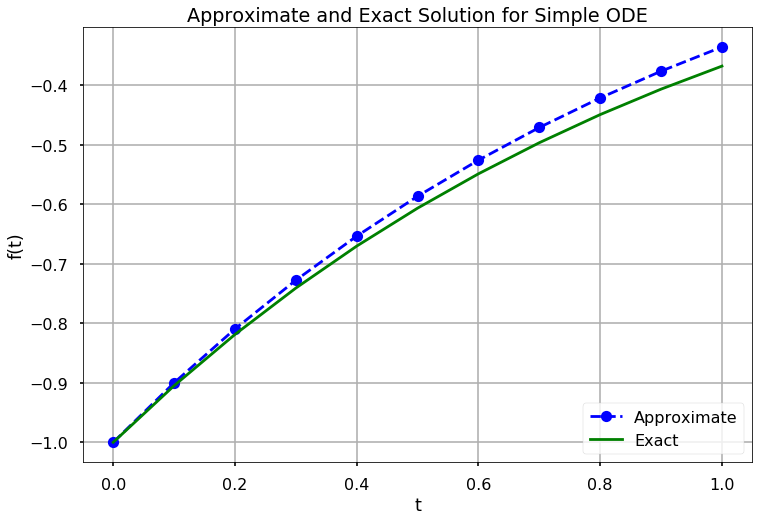
\includegraphics[width=10cm]{mod10sect2pic1}
\end{center}
\end{mysolution}

%In the above figure, we can see each dot is one approximation based on the previous dot in a linear fashion. From the initial value, we can eventually get an approximation of the solution on the numerical grid. If we repeat the process for $h=0.01$, we get a better approximation for the solution:
\begin{myexercise}\label{Comprehensionquiz2}
The differential equation $\frac{df(t)}{dt}=e^{-t}$ with initial condition $f_0=-1$ has the exact solution $f(t)=-e^{-t}$. Approximate the solution to this initial value problem between $0$ and $1$ in increments of $0.01$ using the Explicity Euler Formula. Plot the difference between the approximated solution and the exact solution.
\end{myexercise}
\begin{mysolution}
\end{mysolution}
\begin{boxB}
import numpy as np\\
import matplotlib.pyplot as plt
\end{boxB}

\begin{boxB}
~\\
plt.style.use('seaborn-poster')\\
%matplotlib inline\\
\\
\# Define parameters\\
f = lambda t, s: np.exp(-t) \# ODE\\
h = 0.01 \# Step size\\
t = np.arange(0, 1 + h, h) \# Numerical grid\\
s0 = -1 \# Initial Condition\\
\\
\# Explicit Euler Method\\
s = np.zeros(len(t))\\
s[0] = s0\\
\\
for i in range(0, len(t) - 1):\\
    \hspace*{1cm}s[i + 1] = s[i] + h*f(t[i], s[i])\\
\\
plt.figure(figsize = (12, 8))\\
plt.plot(t, s, 'bo--', label='Approximate')\\
plt.plot(t, -np.exp(-t), 'g', label='Exact')\\
plt.title('Approximate and Exact Solution \textbackslash \\
for Simple ODE')\\
plt.xlabel('t')\\
plt.ylabel('f(t)')\\
plt.grid()\\
plt.legend(loc='lower right')\\
plt.show()
\end{boxB}

\begin{center}
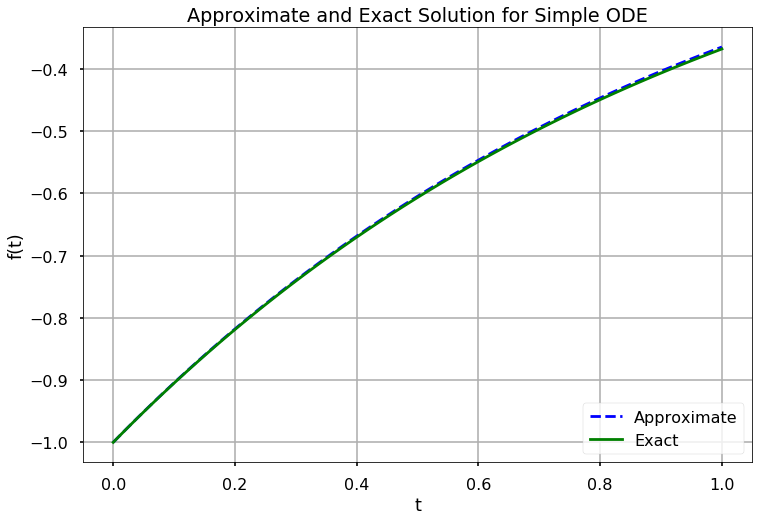
\includegraphics[width=10cm]{CompQuizMod10Sec2Q1}
\end{center}






\section{Numerical Error and Instability}
\activities
Read the reference below on numerical error and instability in indicated web pages and then attempt the subsequent quiz.
\begin{activity}[\cg Reading]
\begin{enumerate}
\item Kong, Q., Siauw, T., Bayen, A., (2020). Python Programming and Numerical Methods. First Edition, Academic Press,  ISBN-13 ‏ : ‎ 978-0128195499 \\
\mylink{https://pythonnumericalmethods.studentorg.berkeley.edu/notebooks/chapter22.05-Predictor-Corrector-Methods.html}
\end{enumerate}
\end{activity}

\begin{myexercise}
Use the Euler Explicit, Euler Implicit, and Trapezoidal Formulas to solve the pendulum equation over the time interval $[0,5]$ in increments of $0.1$ and for an initial solution of $S_0 = \left[\begin{array}{c} 1\\0 \end{array}\right]$. For the model parameters using $\sqrt{\frac{g}{l}} = 4$. Plot the approximate solution on a single graph
\end{myexercise}


\begin{mysolution}     
\begin{boxB}
import numpy as np\\
from numpy.linalg import inv\\
import matplotlib.pyplot as plt\\
\\
plt.style.use('seaborn-poster')\\
\\
\%matplotlib inline 
\end{boxB}
%\end{mysolution}     
%
%\begin{mysolution}     
\begin{boxB}
\# define step size\\
h = 0.1\\
\# define numerical grid\\
t = np.arange(0, 5.1, h)\\
\# oscillation freq. of pendulum\\
w = 4
s0 = np.array([[1], [0]])
\end{boxB}

\begin{boxB}
~\\
m\_e = np.array([[1, h], \\
\hspace*{2cm}[-w**2*h, 1]])\\
m\_i = inv(np.array([[1, -h], \\
\hspace*{2cm}[w**2*h, 1]]))\\
m\_t = np.dot(inv(np.array([[1, -h/2], \\
\hspace*{1cm}[w**2*h/2,1]])), np.array(\\
\hspace*{1.5cm}[[1,h/2], [-w**2*h/2, 1]]))\\
\\
s\_e = np.zeros((len(t), 2))\\
s\_i = np.zeros((len(t), 2))\\
s\_t = np.zeros((len(t), 2))\\
\\
\# do integrations\\
s\_e[0, :] = s0.T\\
s\_i[0, :] = s0.T\\
s\_t[0, :] = s0.T\\
\\
for j in range(0, len(t)-1):\\
\hspace*{1cm}s\_e[j+1, :] = np.dot(m\_e,s\_e[j, :])\\
\hspace*{1cm}s\_i[j+1, :] = np.dot(m\_i,s\_i[j, :])\\
\hspace*{1cm}s\_t[j+1, :] = np.dot(m\_t,s\_t[j, :])\\
\\    
plt.figure(figsize = (12, 8))\\
plt.plot(t,s\_e[:,0],'b-')\\
plt.plot(t,s\_i[:,0],'g:')\\
plt.plot(t,s\_t[:,0],'r--')\\
plt.plot(t, np.cos(w*t), 'k')\\
plt.ylim([-3, 3])\\
plt.xlabel('t')\\
plt.ylabel('$\Theta (t)$')\\
plt.legend(['Explicit', 'Implicit', \textbackslash \\
\hspace*{2cm}'Trapezoidal', 'Exact'])\\
plt.show()\\
\end{boxB}
\end{mysolution}

\begin{figure}[h]
\centering
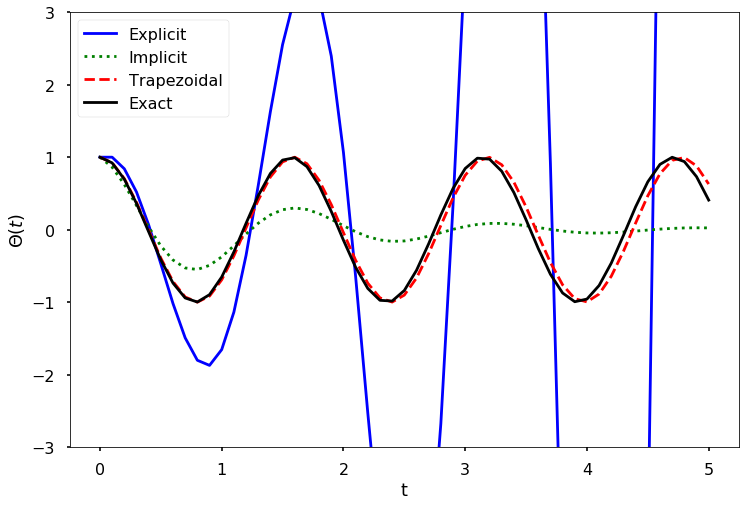
\includegraphics[width=13cm]{Mod10sect2solution}
%\caption{}
%\label{}
\end{figure}


\section{Python ODE Solvers}
%\videolesson
%\begin{selfvideo}[2]
%%LESSON 3: 
%This video presents a discussion on python ODE solver (IVP) and advanced topics. Follow the discussion and then solve the problems in the subsequent quiz.
%\end{selfvideo}
\activities
Read the reference below on python ODE solvers in indicated web pages and then attempt the subsequent quiz.
\begin{activity}[\cg Reading]
\begin{enumerate}
\item Kong, Q., Siauw, T., Bayen, A., (2020). Python Programming and Numerical Methods. First Edition, Academic Press,  ISBN-13 ‏ : ‎ 978-0128195499 \\
\mylink{https://pythonnumericalmethods.studentorg.berkeley.edu/notebooks/chapter22.06-Python-ODE-Solvers.html}
\end{enumerate}
\end{activity}

%\begin{boxB}Question: \end{boxB}
\begin{myexercise}\label{Comprehensionquiz2}
Consider the ODE
\[\frac{dS(t)}{dt} = -S(t)\]
with an initial value of $S_0=1$. The exact solution to this problem is $S(t)=e^{-t}$. Use $solve\_ivp$ to approximate the solution to this initial value problem over the interval $[0,1]$. Plot the approximate solution versus the exact solution, and the relative error over time.
\end{myexercise}

\begin{mysolution}
\begin{boxB}
F = lambda t, s: -s\\
\\
t\_eval = np.arange(0, 1.01, 0.01)\\
sol = solve\_ivp(F, [0, 1], [1], t\_eval=t\_eval)\\
\\
plt.figure(figsize = (12, 4))\\
plt.subplot(121)\\
plt.plot(sol.t, sol.y[0])\\
plt.xlabel('t')\\
plt.ylabel('S(t)')\\
plt.subplot(122)\\
plt.plot(sol.t, sol.y[0] - np.exp(-sol.t))\\
plt.xlabel('t')\\
plt.ylabel('S(t) - exp(-t)')\\
plt.tight\_layout()\\
plt.show()\\
\end{boxB}
\end{mysolution}

\begin{center}
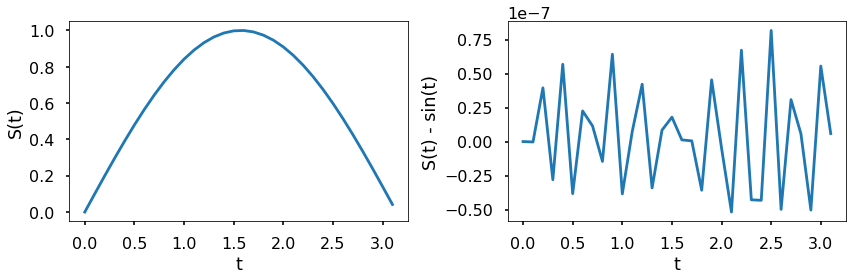
\includegraphics[width=15cm]{Mod10sectionthreesolution}
\end{center}
%
%
%\discussion


\begin{posttest}[\textcolor{red}{End of Module 10 Quiz}]
\item Apply the Euler formula to the first order equation with an oscillating input 
\[\begin{split}
y&=sin(x),\\
 0&\leq x\leq 10.
\end{split}\]

\begin{mysolution}
\item The equation can be approximated using the forward Euler as 
\[\frac{w_{i+1}- w_i}{h} =\sin(x_i).\]
Rearranging the equation gives the discrete difference equation with the unknowns on the left and the known values on the right
 \[w{i+1}=w_i+h\sin(x_i).\]
The Python code bellow implements this difference equation. The output of the code is shown in figure below
\begin{boxB}
\# Numerical solution of a Cosine differential equation\\
import numpy as np\\
import math\\
import matplotlib.pyplot as plt\\
\\
h=0.01\\
a=0\\
b=10\\
\\
N=int(b-a/h)\\
w=np.zeros(N)\\
x=np.zeros(N)\\
Analytic Solution=np.zeros(N)\\
\\
\# Initial Conditions\\
w[0]=1.0\\
x[0]=0\\
Analytic Solution[0]=1.0\\
for i in range (1,N) :\\
\hspace*{1cm}w[i]=w[i 1]+hmath.sin(x[i 1])\\
\hspace*{1cm}x[i]=x[i 1]+h\\
\hspace*{1cm}Analytic Solution[i]=2.0 math.cos(x[i ])\\
\\
fig = plt . figure(figsize=(8,4))\\
\\
\# left hand plot\\
ax = fig.add subplot(1,3,1)\\
plt .plot(x,w,color=’red’)\\
\#ax.legend(loc=’best ’)\\
plt . title( ’Numerical Solution’)\\
\\
\end{boxB}

\begin{boxB}

\#--------right hand plot\\
ax = fig .add subplot(1 ,3 ,2)\\
plt . plot (x, Analytic Solution , color=’blue ’)\\
plt . title ( ’Analytic Solution ’)\\
\\
\#ax. legend( loc=’best ’)\\
ax = fig .add subplot(1 ,3 ,3)\\
plt . plot (x, Analytic Solution w, color=’blue ’)\\
plt . title ( ’Error ’ )\\
\\
\#---------t i t l e , explanatory text and save\\
fig . suptitle ( ’Sine Solution ’ , fontsize=20)\\
plt . tight layout ()\\
plt . subplots adjust (top=0.85)
\end{boxB}
\begin{center}
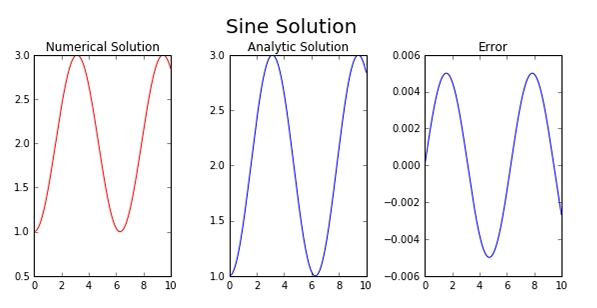
\includegraphics[width=15cm]{EndofMod10QuizQ1solfig}
\end{center}
\end{mysolution}
\item The logistics equation is a simple differential equation model that can be used to relate the change in population $\frac{dP}{dt}$ to the current population, $P$, given a growth rate, $r$, and a carrying capacity, $K$. The logistics equation can be expressed by:
\[\frac{dP}{dt}=rP\left(1-\frac{P}{K}\right)\]
Write a function $my_logistics_eq(t,P,r,K)$ that represents the logistics equation with a return of $dP$. Note that this format allows $my_logistics_eq$ to be used as an input argument to $solve_ivp$. You may assume that the arguments $dP$, $t$, $P$, $r$, and $K$ are all scalars, and $dP$ is the value $\frac{dP}{dt}$ given $r$, $P$, and $K$. Note that the input argument, $t$, is obligatory if $my_logistics_eq$ is to be used as an input argument to $solve_ivp$, even though it is part of the differential equation.

\begin{mysolution}
The logistics equation has an analytic solution defined by:
\[P(t)=\frac{KP_0e^{rt}}{K + P_0(e^{rt}-1)}\]
where $P_0$ is the initial population.

Test case
\begin{boxB}
import numpy as np\\
from scipy.integrate import solve\_ivp\\
import matplotlib.pyplot as plt\\
from functools import partial\\
plt.style.use('seaborn-poster')\\
\\
\%matplotlib inline
\end{boxB}
\begin{boxB}
def my\_logisitcs\_eq(t, P, r, K):\\
\hspace*{1cm}\# put your code here\\
    \\
\hspace*{1cm}return dP\\
\\
dP = my\_logisitcs\_eq(0, 10, 1.1, 15)\\
dP
\end{boxB}

$3.666666666666667$

\begin{boxB}
from functools import partial\\
\\
t0 = 0\\
tf = 20\\
P0 = 10\\
r = 1.1\\
K = 20\\
t = np.linspace(0, 20, 2001)\\
\\
f = partial(my\_logisitcs\_eq, r=r, K=K)\\
sol=solve\_ivp(f,[t0,tf],[P0],t\_eval=t)\\
\\
plt.figure(figsize = (10, 8))\\
plt.plot(sol.t, sol.y[0])\\
plt.plot(t, \textbackslash\\
\end{boxB}

\begin{boxB}
\hspace*{0.5cm}K*P0*np.exp(r*t)/(K+P0*(np.exp(r*t)-1)),'r:')\\
plt.xlabel('time')\\
plt.ylabel('population')\\
\\
plt.legend(['Numerical Solution', \textbackslash\\
\hspace*{2cm}'Exact Solution'])\\
plt.grid(True)\\
plt.show()\\
\end{boxB}

\begin{center}
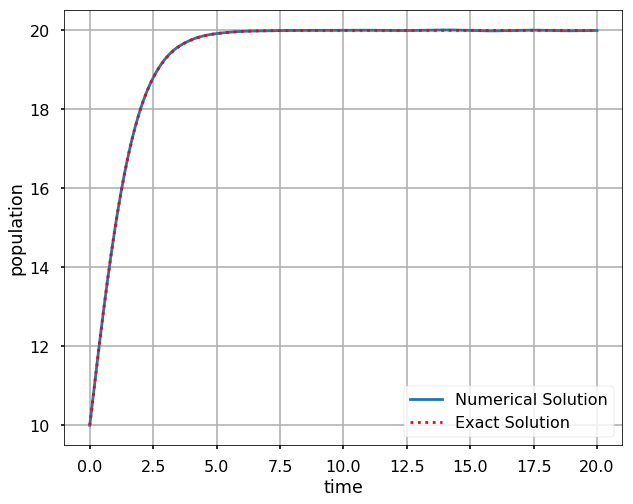
\includegraphics[width=11cm]{EndofModquizqn3sol}
\end{center}
\end{mysolution}



\end{posttest}

%share your understanding of properties of functions and their applications to solving rates of change problems in physical phenomenon 


%\end{actsoln}

\takehome

\comy{You are now at the last part of this module. Your  task is to do a self-reflection on your learning experience.}



\references
\begin{refenumerate}
\item Kong, Q., Siauw, T., Bayen, A., (2020). Python Programming and Numerical Methods. First Edition, Academic Press,  ISBN-13 ‏ : ‎ 978-0128195499 \\
\mylink{https://pythonnumericalmethods.studentorg.berkeley.edu/notebooks/Index.html}
%chapter 1 pg 7-36 functions\\
%chapter 1 pg 51-83 limits and continuity\\
%chapter 1 pg 45-50 rates of change\\
%chapter 2 pg 108-120 the derivative\\
%\item Mendelson, E. (2022). Schaum's Outline of Calculus. McGraw-Hill Education.
%chapter 6 51-55 functions
%chapter 7 59-65 limits
%chapter 8 69-74 continuity
%chapter 9 77-81 derivative
%\item Calculus \mylink{https://math.libretexts.org/Bookshelves/Calculus}
%\item Chris McMullen, 2021, Essential Calculus Skills Practice Workbook with Full Solutions, Zishka Publishing, ISBN 978-1-941691-24-3
%\item R. Adams and C. Essex, 2021, Calculus: A complete Course, Addison Wesley, ISBN 13: 978-0135732588
%\item P. Abbott and H. Neill, 2018, Calculus: A Complete Introduction: The Easy Way to Learn Calculus (Teach Yourself), ISBN 13: 978-1473678446
\end{refenumerate}





%\wrapup
%To wrap-up, answer the following questions:
%
%\begin{enumerate}
%\item 
%%when do we say that a limit of a function exists?
%%\item how do we remove discontinuity in functions?
%%\item what is the relationship between the gradient of the tangent line and the derivative?
%\end{enumerate}
















%\newpage

%\facilitation


%
\begin{center}
    {\Large \textbf{FUNCTIONS OF SEVERAL VARIABLES}}\\[2mm]
(DEFINITION, DOMAIN, RANGE, GRAPHS AND LEVEL CURVES) \\[4mm]

\mycenterbox{5 minute review}%\\[4mm]
Recap the definition of a function of several variables, and the meaning of domain, range, graph and level curves of functions of several variables.
\end{center}
\mycenterbox{Warm-up.}%\\[4mm]
\problemAnswer{
Match the function with its graph (labeled I–VI).Give reasons for your choices
\begin{multicols}{3}
\begin{enumerate}[label=(\alph*)]
\item $f(x,y)=|x|+|y|$\\[4mm]
\item $f(x,y)=|xy|$
\item $f(x,y)=\frac{1}{1+x^2+y^2}$\\2mm]
\item $f(x,y)=(x^2-y^2)^2$
\item $f(x,y)=(x-y)^2$\\[4mm]
\item $f(x,y)=\sin(|x|+|y|)$
\end{enumerate}
\end{multicols}

\begin{center}
%\centering
\includegraphics[width=10cm]{MCTutorial1Q1.JPEG}
\end{center}
%\tcbox[tcbox raise base]{Warm-up}
 
%\begin{flushright}
%\begin{tikzpicture}
%    % A body
%
%
%    % Non-rectangle shapes must be drawn as polygone
%    \begin{scope}[shift={(3,0)}]
%        \draw  (0,0.5) -- (0,4) -- (.5,4) -- (.5,4.5) -- (1.,4.5) -- (4.,4.5) --(4.,4)-- (4.5,4) --(4.5,0.5) --(4.0,0.5)--(4.0,0.0)-- (.5,0) --(0.5,0.5) -- cycle;
%        % Draw symmetry lines
%        \draw [symmetry] (.5, 0.5) -- (.5,4.0);
%        \draw [symmetry] (4, 0.5) -- (4,4.0);
%        \draw [symmetry] (.5,4.0) -- (4,4.0);
%         \draw [symmetry] (.5, 0.5) -- (4, 0.5);
%        % Dimensions
%        \draw (4.5,0) -- ++(0.5,0) coordinate (D1) -- +(5pt,0);
%        \draw (4.5,4.5) -- ++(0.5,0) coordinate (D2) -- +(5pt,0);
%        \draw [dimen] (D1) -- (D2) node {6cm};
%       
%        
%        \draw (0.0,5) -- ++(0,0.5) coordinate (D1) -- +(0,+5pt);
%        \draw (0.5,5) -- ++(0,0.5) coordinate (D2) -- +(0,+5pt);
%        \draw [dimen,-] (D1) -- (D2) node [above=5pt] {$x$ cm};
%        \draw [dimen,<-] (D1) -- ++(-5pt,0);
%        \draw [dimen,<-] (D2) -- ++(+5pt,0);
%    \end{scope}
%\end{tikzpicture}
%\end{flushright}

}


\mycenterbox{Problems.}%

%\begin{center}
%\tcbox[tcbox raise base]{ Problems. Choose from the below}
%\end{center}
\problem{Exploring functions}%
\begin{enumerate}[(a)]
\item Are the following functions even, odd, or neither? What can you say
about their range?
\begin{multicols}{4}
 \begin{enumerate}[(i)]
\item $\displaystyle \frac{3x}{x^2+2}$
\item $\displaystyle \cos x+3$
\item $\displaystyle \frac{2x^3}{\cos x+3}$
\item $\displaystyle \frac{3x^4+2x^2}{\sin x+4}$
\end{enumerate}
\end{multicols}
\item Consider the functions $\sin^n x$ and $\cos^n x$, where $n$ is a positive integer.
Which are odd, which are even, and what are their periodicities?
\item What is the periodicity of $f(x) = 2 \cos x+\sin 2x$? Is it even/odd/neither?

\end{enumerate}

\problem{Cubic functions} 
Show that $x-1$ is a factor of the cubic function%
$$P(x)=x^3-2x^2-5x+6,$$
and  find the quadratic factor $Q(x)$ such that $P(x) = (x -1)Q(x)$. Factorise
$Q(x)$ and hence sketch $P(x).$

%\newpage
\problem{Sigmoid functions*.}%
For positive integers $n$, consider the family of functions
$$\displaystyle f_n= \frac{x^n}{2^n+x^n}.$$
\begin{enumerate}[(a)]
\item What are appropriate domains and ranges for $f_n(x)$? Do they depend on $n$?

\item Is $f_n(x)$ even, odd, or neither? Does this depend on $n$?

\item Show that for $x\geq 0$, $f_n(x)$ are strictly increasing functions and that
$0\leq f_n(x) < 1.$
\item What is the value of $f_n(2)$? Does it depend on $n$?

\item By considering the values of $f_n(1.9)$ and $f_n(2.1)$ for $n = 2, 4, 8, 16, 32$ and
$64$, show that the graph of $f_n(x)$ for $x\ge 0$ is an increasing sigmoid (that
is, $S$-shaped) function that approaches a step function as $n\rightarrow \infty$.
\end{enumerate}

\mycenterbox{Selected answers and hints}%

For the warm-up, $V(x)=4x(3-x)^2$. Writing $x=1+\epsilon$, we get
$$V = 4(1 +\epsilon)(3- (1+\epsilon))^2=4(4-\epsilon^2(3-\epsilon)).$$
If $-1<\epsilon<2$ then $\epsilon^2 (3-\epsilon)\ge 0$, with equality when $\epsilon=0$. Thus the maximum
value of $V$ occurs when $\epsilon= 0$, i.e. $x = 1\rm{cm}$.

\begin{enumerate}
\item 
\begin{enumerate}[(i)]
\item Odd. The range is the interval  $[-\frac{3}{4}\sqrt{2},\; \frac{3}{4}\sqrt{2}]$
\item Even. The range is the interval $[2, 4]$.
\item Odd. The range is all of $\mathbb R$.
\item Neither. (For example, writing $\displaystyle \frac{5}{\sin x+4}$ we have $\displaystyle f(1)= \frac{5}{\sin (1)+4} \equiv 1.032 (3\rm{dp})$ which is neither $f(1)$ nor $-f(1)$.)\\[4mm]
The range is the nonnegative reals $[0,\infty)$

\end{enumerate}
\end{enumerate}










